Pada Bab Ini akan membahas mengenai metode entropy,
Kelebihan dan kekurangan metode entropy 
Penjelasan dari rumus metode entropy
Penjelasan mengenai cara penggunaan metode entropy
Jenis data yang bisa diolah menggunakan metode entropy kemudian penggunaan entropy pada sistem
\pagebreak

\section{Metode Entropy}

Metode entropy merupakan metode yang di gunakan untuk menentukan tingkat kepentingan dari keriteria atau pembobotan untuk keriteria  selain itu metode ini juga dapat di gunakan untuk menentukan tingkat kepentingan awal atau bobot awal dari keriteria \cite{harahap2017penerapan}, \cite{chai2018new}. Sehingga walaupun di perhitungan awal bobot dari nilai entropy kecil pada suatu keriteria milaslkan dikarenakan variasi data yang kecil pada keriteria tersebut, namun jika keriteria tersebut di anggap penting oleh pengambil keputusan maka dia dapat memberikan bobot yang tinggi pada criteria tersebut, kedua bobot tersebut kemudian dapat di kalkulasikan sehingga mendapatkan nilai entropy akhir Lalu metode ini dapat menyelidiki keserasian dalam diskriminasi diantara sekumpulan data\cite{malekian2016application} . Nilai-nilai alternatif pada kriteria tertentun digambarkan dalam secision matrix (DM). dengan menggunakan metode entropy dengan variasi nilai tertinggi akan mendapatkan nilai tertinggi \cite{meiriza2019implementasi}.

Pada buku ini salah satu rumus entropy yang akan di bahas yaitu metode entropy shannons atau shannons entropy, yang memiliki persamaan atau rumus seperti pada gambar \ref{r1} berikut ini:

\begin{figure}[h]
	\centerline{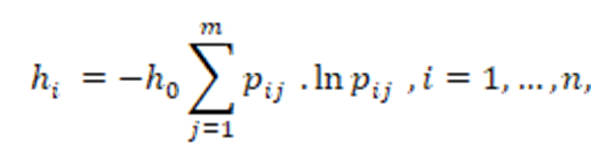
\includegraphics[width=0.6\textwidth]{figures/rumus/1.png}}
	\caption{Rumus Shanon's Entropy}
	\label{r1}
\end{figure}


Rumusan tersebut ditemukan Pada tahun 1948 Claude E. Shannon yang memperkenalkan entropy informasi sehingga sekarang sering di sebut dengan Entropy shannon, Selain digunakan untuk membobotkan setiap keriteria dari alternatif Metode ini juga dapat di gunakan untuk mengevaluasi bobot pada dasar subjektif dan objektif bobot \cite{wu2011determination}.

Maka dari itu berikut ini merupakan ada beberapa ketentuan data yang bisa di terapkan pada metode entropy ini, berikut merupakan ke tentuan ketentuannya:
\begin{enumerate}

\item Data dapat berupa data kualitatif 
\item Data juga dapat berupa data kuantitatif
\item Data-data tersebut harus dapat terukur 
\item Satuan untuk setiap keriteria boleh berbeda
\end{enumerate}
\pagebreak

\subsection{Kelebihan dan Kekurangan Entropy}

Setiap metode pasti ada kekurangan dan kelebihan maka dari itu berikut merupakan beberapa kekurangan dan kelebihan dari metode entropy:

Kelebihan dari metode ini diantaranya:\par
\begin{itemize}
\item Dapat membobotkan data baik itu data kualitatif atau data kuantitatif dengan catatan data tersebut dapt terukur atau memiliki nilai

\item Memberikan bobot awal untuk pengambilan keputusan
\end{itemize}
Kekurangan dari metode diantaranya:\par
\begin{itemize}
\item Hasil dari pembobotan bisa sangat kecil maupun sangat besar tergantung pada data nominal data yang di gunakan atau fariasi data yang kecil maupun besar.
\end{itemize}
\subsection{Tahapan Penggunaan Metode Entropy}
	Setiap metode pasti ada langkah-langkah atau tahapan untuk melakukan perhitungan dengan metode tersebut, begitupula dengan metode entropy terdapat tahapan-tahapan untuk menggunakan metode tersebut, maka dari itu berikut merupakan thapan-tahapan untuk menggunkan metode entropy:

\begin{enumerate}
\item Normalisasi terlebih dahulu data setiap keriteria, menggunakan persamaan atau sesuai dengan rumus pada gambar \ref{r2} berikut:

\begin{figure}[h]
	\centerline{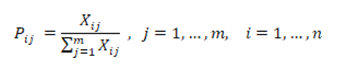
\includegraphics[width=0.6\textwidth]{figures/rumus/2.png}}
	\caption{Rumus Normalisasi Data}
	\label{r2}
\end{figure}

adapun arti dari rumus pada gambar tersebut seperti berikut:
\begin{itemize}
\begin{figure}[h]
	\centerline{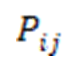
\includegraphics[width=0.1\textwidth]{figures/rumus/2-1.png}}
	\caption{Simbol Data delah dinormalisasi}
	\label{r3}
\end{figure}
\item pada gambar \ref{r3} merupakan simbol rumus dari data yang telah di normalisasi.
\pagebreak
\begin{figure}[h]
	\centerline{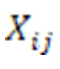
\includegraphics[width=0.1\textwidth]{figures/rumus/2-2.png}}
	\caption{Simbol Nilai Pada satu kolom}
	\label{r4}
\end{figure}
\item Pada gambar \ref{r4} merupakan simbol dari nilai yang terdapat pada satu kolom
\begin{figure}[h]
	\centerline{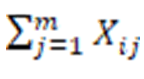
\includegraphics[width=0.1\textwidth]{figures/rumus/2-3.png}}
	\caption{Nilai total dari satu baris}
	\label{r5}
\end{figure}
\item  Pada gambar \ref{r5} merupakan simbol dari nilai total data yang berada pada satu baris yang sama.
\begin{figure}[h]
	\centerline{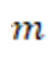
\includegraphics[width=0.1\textwidth]{figures/rumus/2-4.png}}
	\caption{Simbol Jumlah Baris Alternatif}
	\label{r6}
\end{figure}
\item pada gambar \ref{r6} merupaka simbol dari jumlah alternatif
\end{itemize}
agar lebih jelas dapat di lihat pada ilustrasi pada tabel 2.1 berikut:

\begin{table}[h]
\caption{Ilustrasi data yang dinormalisasi}
\centering
\begin{tabular}{|c|c|c|c|c|}
\hline
Alternatif & Kriteria 1 & Kriteria 2 & Kriteria 3 \\
\hline
1   & Xij & Xij& Xij\\
\hline
2   & Xij & Xij& Xij\\
\hline
3   & Xij & Xij& Xij\\
\hline
4   & Xij & Xij& Xij\\
\hline
5   & Xij & Xij& Xij\\
\hline
\end{tabular}
\label{as}
\end{table}

Dimana nilai total dari kriteria 1 yaitu Xij+Xij+Xij+Xij+Xij \par

sehingga contoh untuk mencari nilai pada alternatif 1 dan keriteria 1 seperti berikut:\par

Xij pada kolom ke satu baris ke satu dibagi dengan nilai total keriteria ke satu

\pagebreak

\item Setelah menormalisasi data tersebut lakukan perhitungan entropy menggunakan perasamaan pada gambar \ref{rr1}:

\begin{figure}[h]
	\centerline{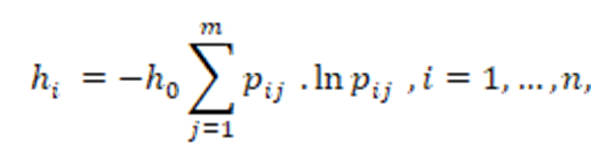
\includegraphics[width=0.6\textwidth]{figures/rumus/1.png}}
	\caption{Rumus Shanon's Entropy}
	\label{rr1}
\end{figure}

Kemudian untuk arti dari rumus tersebut sebagai berikut:
\begin{itemize}
\begin{figure}[h]
	\centerline{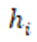
\includegraphics[width=0.05\textwidth]{figures/rumus/3.png}}
	\caption{Simbol Nilai Entropy awal}
	\label{rr2}
\end{figure}
\item pada gambar \ref{rr2} tersebut merupakan tanda atau sintaks untuk Nilai Entropy Awal

\begin{figure}[h]
	\centerline{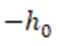
\includegraphics[width=0.1\textwidth]{figures/rumus/3-1.png}}
	\caption{Simbol Nilai Koefisiaen}
	\label{rr3}
\end{figure}

\item pada gambar \ref{rr3} tersebut merupakan tanda atau sintaks dari nilai koefisien, untuk mendapatkan nilai koefisien dapat dilakukan dengan menggunakan rumus pada gambar \ref{rr4}

\begin{figure}[h]
	\centerline{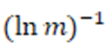
\includegraphics[width=0.12\textwidth]{figures/rumus/3-2.png}}
	\caption{Rumus Nilai Koefisien}
	\label{rr4}
\end{figure}

\item adapun penjelasan untuk rumus koefisien seperti berikut:

\begin{figure}[h]
	\centerline{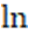
\includegraphics[width=0.05\textwidth]{figures/rumus/3-3.png}}
	\caption{Simbol Nilai Logaritma}
	\label{rr5}
\end{figure}

pada gambar \ref{rr5} yaitu niali logaritma dari jumlah baris atau total alternatif
\pagebreak
\begin{figure}[h]
	\centerline{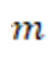
\includegraphics[width=0.05\textwidth]{figures/rumus/2-4.png}}
	\caption{Simbol Jumlah Alternatif}
	\label{rr6}
\end{figure}

pada gambar \ref{rr6} yaitu jumlah alternatif yang ada pada data.

\begin{figure}[h]
	\centerline{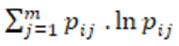
\includegraphics[width=0.4\textwidth]{figures/rumus/3-4.png}}
	\caption{Nila Total hasil kali data normalisasi}
	\label{rr7}
\end{figure}

pada gambar \ref{rr7} merupakan nilai total data normalisasi yang telah dikalikan dengan nilai normalisasi yang sebelumnya di kalikan dengan nilai normalisasi.\par
\end{itemize}

kemudian untuk tahapan implementasi dari rumus tersebut sebagai berikut:

\begin{itemize}
\item pertama cari nilai cari nilai dari koefisien dengan cara mempraktikan rumus koefisien, pada rumus tersebut terdapat pangkat -1 yang berarti 1 dibagi, sehingga dalam mengimplementasikan rumus koefisien yaitu dengan cara 1 di bagi dengan nilai log dari total baris kemudian nilainya ubah menjadi minus, hal ini di karenakan sudah ketentuan dari rumusan entropy.

\item kedua cari nilai perkalian data yang telah di normalisasi dengan data normalisasi yang sudah di kalikan dengan nilai log, agar lebih jelas contoh penempatannya seperti pada tabel 2.2 berikut ini:

\begin{table}[h]
\caption{Ilustrasi Perkalian data yang telah di normalisasi}
\centering
\begin{tabular}{|c|c|c|c|c|}
\hline
Alternatif & Kriteria 1 & Kriteria 2 & Kriteria 3 \\
\hline
1   & Pij * ln Pij & Pij * ln Pij & Pij * ln Pij \\
\hline
2   & Pij * ln Pij  & Pij * ln Pij & Pij * ln Pij \\
\hline
3   & Pij * ln Pij  & Pij * ln Pij & Pij * ln Pij \\
\hline
4   & Pij * ln Pij  & Pij * ln Pij & Pij * ln Pij \\
\hline
5   & Pij * ln Pij  & Pij * ln Pij & Pij * ln Pij \\
\hline

\end{tabular}
\label{table2}
\end{table}

\item setelah itu cari nilai total dari setiap baris keriteria dengan cara menambahkan data yang ada pada setiap baris yang terdapat pada setiap kriteria.

\item kemudian jika semua nilai total telah di dapatkan, kalikan nilai total tersebut dengan nilai koefisien yang sudah dalam keadaan negatif, untuk hasilnya pasti akan bernilai positif.
\end{itemize}

\pagebreak

\item Cari nilai bobot entropy akhir dengan menggunakan rumus pada gamabr \ref{rrr1} berikut:

\begin{figure}[h]
	\centerline{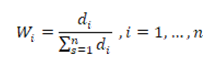
\includegraphics[width=0.6\textwidth]{figures/rumus/4.png}}
	\caption{Nila Total hasil kali data normalisasi}
	\label{rrr1}
\end{figure}
kemudian untuk penjelasan rumus pada gambar \ref{rrr1} tersebut sebagai berikut:

\begin{itemize}
\begin{figure}[h]
	\centerline{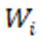
\includegraphics[width=0.05\textwidth]{figures/rumus/4-1.png}}
	\caption{Simbol Bobot Entropy}
	\label{rrr2}
\end{figure}
\item Pada gambar \ref{rrr2} merupakan gambar dari simbol bobot entropy
\begin{figure}[h]
	\centerline{
\includegraphics[width=0.05\textwidth]{figures/rumus/4-2.png}}
	\caption{Simbol Keriteria Ke sekian}
	\label{rrr3}
\end{figure}
\item Pada gambar \ref{rrr3} merupakan gambar dari simbol keriteria ke sekian
\begin{figure}[h]
	\centerline{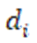
\includegraphics[width=0.05\textwidth]{figures/rumus/4-3.png}}
	\caption{Nilai Hasil Kurang antara satu dengan nilai entropy pertama}
	\label{rrr4}
\end{figure}
\item Pada gambar \ref{rrr4} merupakan gambar dari simbol hasil kurang antara satu dengan nilai entropy yang pertama
\begin{figure}[h]
	\centerline{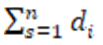
\includegraphics[width=0.13\textwidth]{figures/rumus/4-4.png}}
	\caption{Nila Total dari hasi kurang}
	\label{rrr5}
\end{figure}
\item Pada gambar \ref{rrr5} merupaka simbol dari nilai total hasil pengurangan antara 1 (satu) dengan bobot awal
\end{itemize}

Untuk tahapan mencari nilai total dapat di lakukan dengan cara seperti berikut ini:

\begin{itemize}
\item setelah nilai total dari hasil perkalian data yang telah di normalisasi dan nilai koefisien ditemukan, data tersebut dijadikan sebagai pengurang dari niali 1 (satu), nilai satu tersebut merupakan nilai ketentuan dari rumus bobot entropy total.

\item kemudian jika semua nilai telah di temukan dari setiap keriteria maka cari nilai total dari hasil pengurangan yang di lakukan pada setiap keriteria, sehingga di dapatkan nilai total dari hasil pengurangan tersebut.

\item jika nilai total sudah di temukan maka nilai total tersebut menjadi pembagi untuk setiap data yang telah di kurangi.
\end{itemize}

\textbf{Catatan :}\par
\textit{Pada saat mencari nilai bobot akhir dilakukan pembagian dari nilai pengurangan dari setiap criteria dengan nilai total dari semua pengurangan dari semua keriteria, atau untuk lebih jelasnya dapat di lihat pada contoh perhitungan entropy pada BAB 3}
\end{enumerate}

\subsection{Contoh Kasus Dalam Penerapan Metode Entropy}

Dalam penerapannya metode ini dapat di terapkan pada beberapa kasus pengambilan keputusan, contohnya seperti pada kasus pengambilan keputusan untuk memilih siswa terbaik \cite{majdi2017penerapan}, kemudian dalam pembobotan untuk memilih supplier bahan baku \cite{saputra2016usulan}, selain itu metode ini juga dapat di terapkan pada kasus untuk pemilihan perawatan saluran air \cite{brankovic2018comparative} selain itu metode ini juga dapat di gunakan untuk mengevaluasi sesuatau contohnya seperti mengevaluasi hasil operasi perusahaan jaringan listrik \cite{wu2018comprehensive}, kemudian untuk contoh lainnya metode entropy juga dapat digunakan untuk mencari bobot untuk perangkingan atau urutan \cite{harahap2017penerapan}.

\section{Implementasi Metode Entropy Pada Sistem}

 Pada contoh sistem yang di buat pada aplikasi ini metode entropy di terapkan pada bagian menu Proses entropy, namun sebelum masuk ke menu tersebut terlebih dahulu untuk setiap user pengguna sistem melengkapi terlebih dahulu data yang terdapat pada menu data alternatif, hal ini disebabkan karena data yang dilakukan pembobotan menggunakan metode entropy ini menggunakan data yang terdapat pada tabel alternatif. Jika data yang terdapat pada menu data alternetif telah ada dan lebih dari 2 (dua) data, maka proses entropy dapat di lakukan. kemudian agar lebih jelas untuk tahapan-tahapan proses entropy pada sistem seperti berikut ini:
\pagebreak
\begin{enumerate}
\item klik menu Proses entropy seperti pada gambar \ref{ro1} dan gambar \ref{ro2} berikut 

\begin{figure}[h]
	\centerline{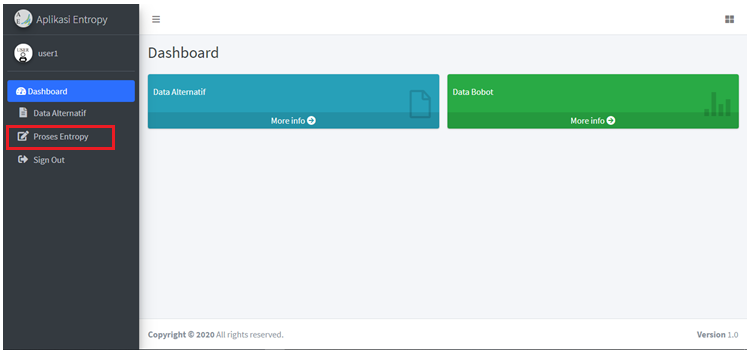
\includegraphics[width=0.9\textwidth]{figures/pje/1.png}}
	\caption{Menu entropy pada halaman utama admin}
	\label{ro1}
\end{figure}

\begin{figure}[h]
	\centerline{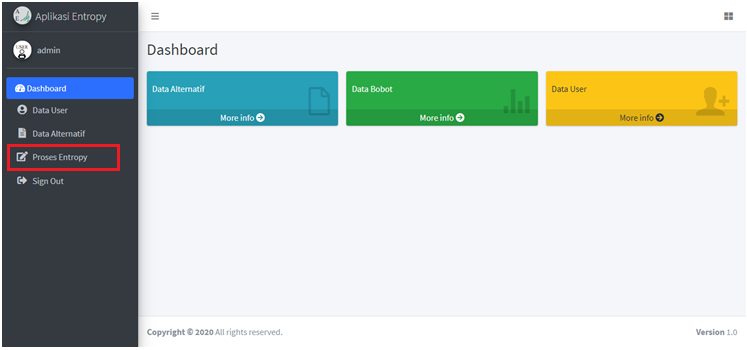
\includegraphics[width=0.9\textwidth]{figures/pje/2.png}}
	\caption{Menu Entropy pada halaman utama selain admin}
	\label{ro2}
\end{figure}
\pagebreak
\item kemudian jika telah masuk ke menu proses entropy masukan id user pada form seperti pada gambar \ref{ro3} berikut ini.

\begin{figure}[h]
	\centerline{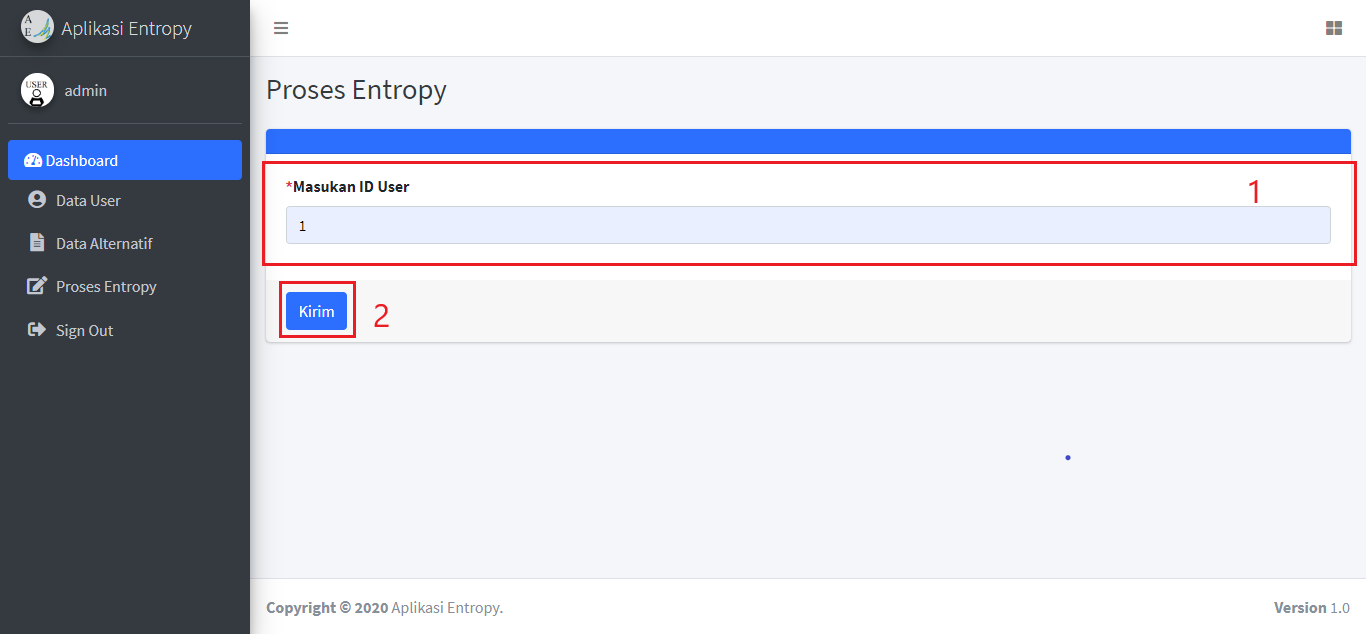
\includegraphics[width=0.90\textwidth]{figures/pje/3.png}}
	\caption{Form insert user id}
	\label{ro3}
\end{figure}

\item setelah itu klik tombol kirim pada form tersebut kemudian hasil dari perhitungan entropy akan muncul seperti pada gambar \ref{ro4} berikut 

\begin{figure}[h]
	\centerline{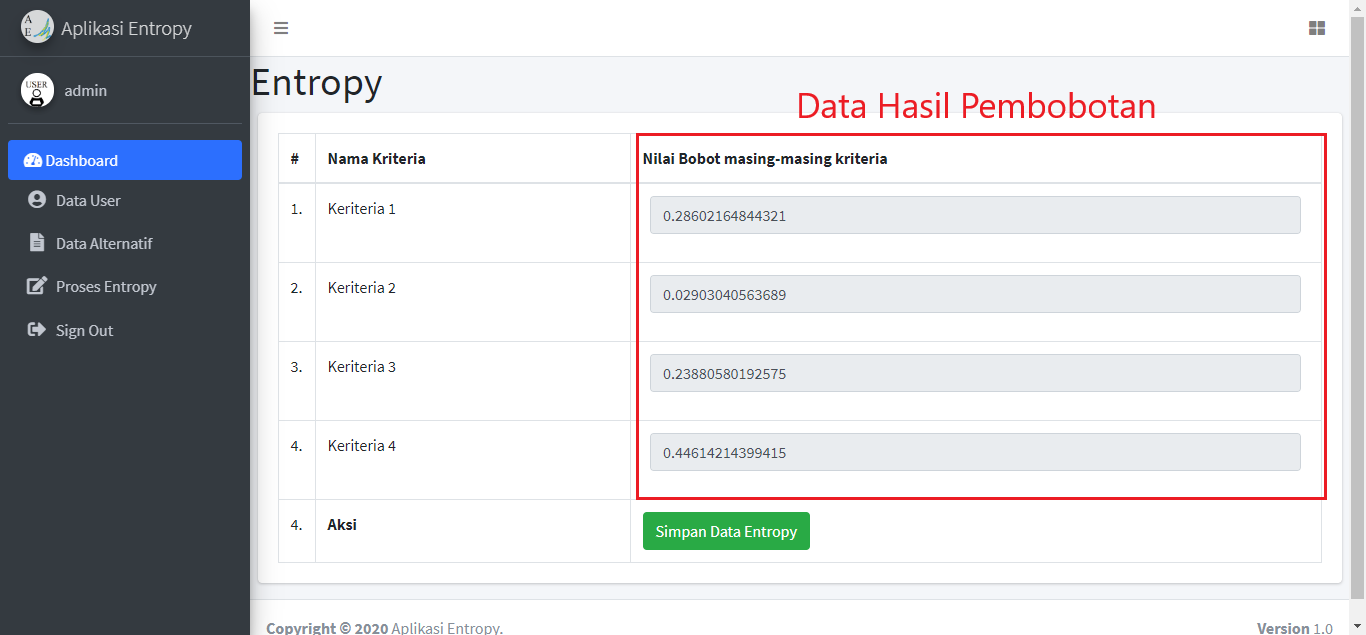
\includegraphics[width=0.90\textwidth]{figures/pje/4.png}}
	\caption{Hasil Perhitungan Entropy}
	\label{ro4}
\end{figure}
\pagebreak
\item jika data bobot hasil entropy dirasa di butuhkan atau akan segera di gunakan bisa menekan tombol simpan data entropy seperti pada gambar \ref{ro5} berikut 

\begin{figure}[h]
	\centerline{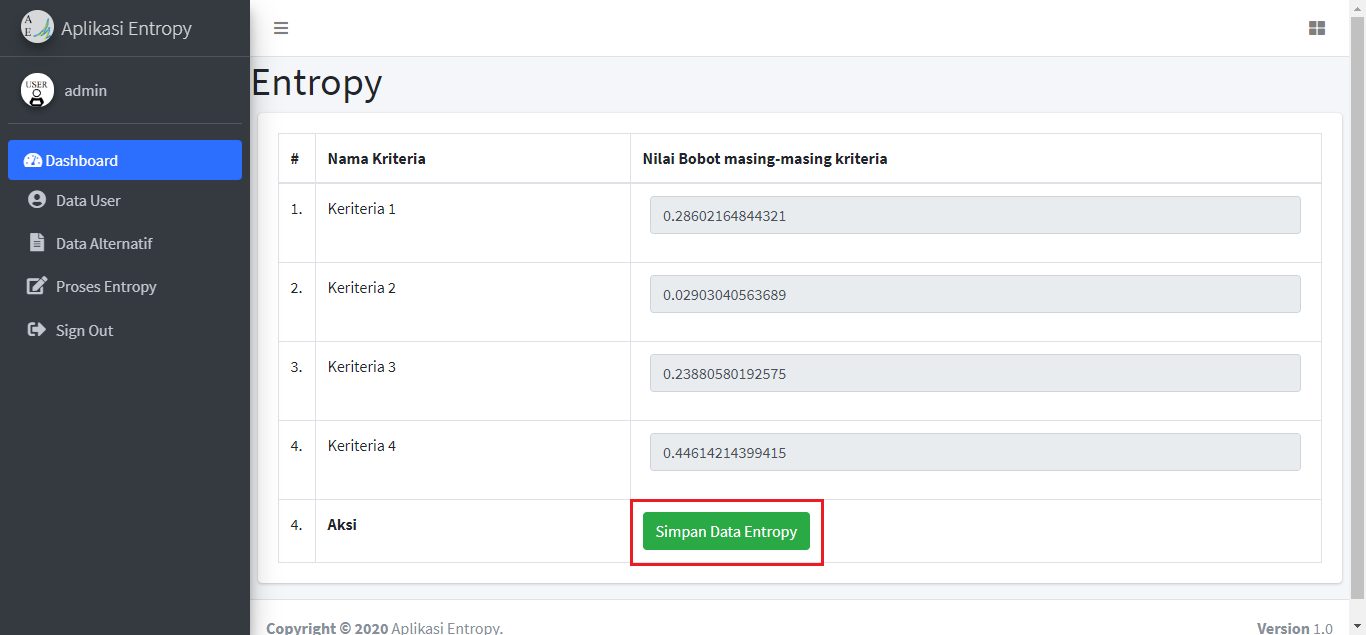
\includegraphics[width=0.80\textwidth]{figures/pje/5.png}}
	\caption{Menyimpan Data Entropy}
	\label{ro5}
\end{figure}

\item maka hasil data yang telah disimpan akan masuk ke basis data sistem yang hasilnya terdapat pada menu data bobot seperti pada gambar \ref{ro6} berikut

\begin{figure}[h]
	\centerline{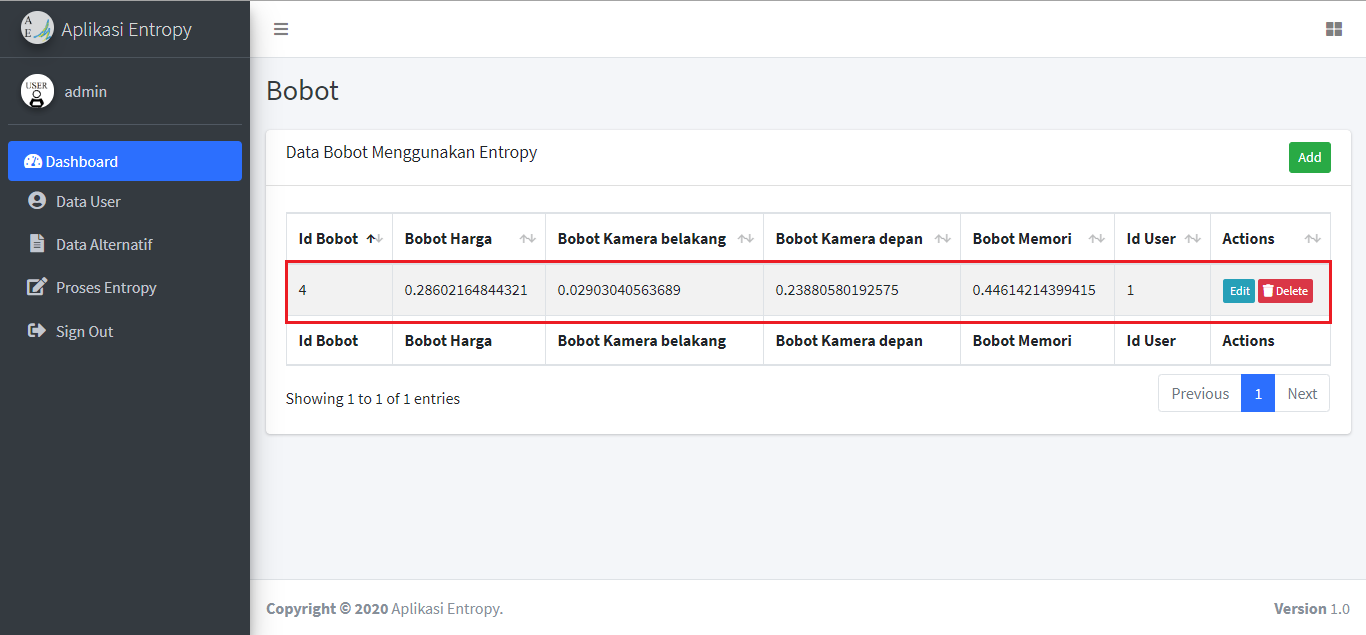
\includegraphics[width=0.80\textwidth]{figures/pje/6.png}}
	\caption{Data Bobot yang telah di simpan}
	\label{ro6}
\end{figure}
\end{enumerate}

\textbf{Catatan :}\par
\textit{Pada tahapan tersebut sebenarnya ada perbedaan untuk user admin dan user pengguna sistem biasa atau yang levelnya di bawah admin, jika user yang login ke sistem bukan user admin maka tidak perlu melakukan input id user hanya perlu menekan menu proses entropy maka akan muncul hasil seperti pada tahapan ke 3, kemudian untuk proses menyimpan data entropy sama seperti pada user admin. Selain itu Proses ini hanya dapat dilakukan jika data lebih dari dua atau minimal dua baris data.}

